\chapter{Data and measurement}\label{ch:data}
\chapterlead{All data come from public exchange archives and are built by scripts that check each step against the
exchange's own rules. This chapter describes the sources and checks, the bans, the futures-cash basis, the other outcomes
and a constraint index for every listed stock.}

\section{Sources}
All data come from public archives, downloaded and parsed with scripts so that every step can be repeated
(the full version of the thesis).
\begin{table}[t]
\caption[Data sources]{Every series comes from a public archive}\label{tab:sources}
\exsub{Sources, content and coverage}
\small\begin{tabularx}{\textwidth}{@{}K{4.3cm}L>{\raggedright\arraybackslash}p{2.9cm}@{}}
\toprule
\thd{Source} & \thd{Content} & \thd{Coverage} \\
\midrule
NSE combined open interest files & MWPL, open interest, futures-equivalent open interest (from Oct 2025), next-day status & Feb 2010 to Oct 2026 \\ \rowrule
NSE securities-in-ban lists & Official ban list & Feb 2010 to Oct 2026 \\ \rowrule
NSE F\&O and cash bhavcopies, delivery files & Prices, traded value and quantity, contracts, open interest, delivery & 2015 to Oct 2026 \\ \rowrule
NSE corporate actions & Dividends, splits, bonuses and other events with ex-dates & 2014 to 2026 \\ \rowrule
NSE announcements, results filings, board meetings & First dissemination time of quarterly results & 2014 to 2026 \\ \rowrule
NSE SLB bhavcopies & Daily securities-lending trades and fees & 2015 to Oct 2026 \\ \rowrule
AMFI & Half-yearly average market capitalisation lists; monthly arbitrage-fund flows and assets & 2017 to 2026; Apr 2018 to Sep 2026 \\ \rowrule
OECD via FRED & Three-month interbank rate (monthly) & 2011 to 2026 \\
\bottomrule
\end{tabularx}
\exsource{Source: National Stock Exchange of India archives; Association of Mutual Funds in India; OECD Main Economic Indicators via FRED.}
\end{table}

\section{Checks}
Of the 11,764 daily ``no fresh positions'' flags, 11,753 (99.9\%) match the next day's official ban list, and utilisation
was above 95\% the day before 99.4\% of ban spells began. Results announcements are dated from the exchange's first
dissemination time, which covers 98\% to 100\% of F\&O stock-quarters.

\section{Bans}
\begin{table}[t]
\caption[F\&O bans by year, 2015 to 2026]{Bans are frequent, concentrated in a few stocks, and longer under the new rule}\label{tab:bans}
\exsub{F\&O stocks, banned stocks, ban spells and ban stock-days by year}
\centering{\footnotesize\setlength{\tabcolsep}{4pt}\begin{tabular}{lrrrrrr}
\toprule
Year & \shortstack[r]{F\&O stocks\\(avg per day)} & \shortstack[r]{Stocks\\banned} & \shortstack[r]{Ban\\spells} & \shortstack[r]{Ban\\stock-days} & \shortstack[r]{Median spell\\(days)} & \shortstack[r]{Longest spell\\(days)} \\
\midrule
2015 & 154 & 16 & 69 & 367 & 4 & 21 \\
2016 & 172 & 27 & 136 & 645 & 4 & 17 \\
2017 & 200 & 43 & 287 & 1586 & 5 & 24 \\
2018 & 206 & 38 & 162 & 810 & 4 & 31 \\
2019 & 176 & 23 & 86 & 508 & 4 & 17 \\
2020 & 140 & 40 & 178 & 756 & 3 & 13 \\
2021 & 163 & 26 & 162 & 789 & 4 & 16 \\
2022 & 196 & 23 & 100 & 457 & 4 & 13 \\
2023 & 187 & 41 & 193 & 942 & 4 & 17 \\
2024 & 185 & 49 & 289 & 1656 & 5 & 22 \\
2025 & 216 & 37 & 94 & 556 & 5 & 15 \\
2026$^{a}$ & 209 & 10 & 33 & 342 & 10 & 29 \\
\midrule
2015 to 2026 & 183 & 141 & 1789 & 9414 & 4 & 31 \\
\bottomrule
\end{tabular}
}
\exsource{$^{a}$ January to 27 October 2026. Spells are counted in the year they start. Source: NSE securities-in-ban lists and F\&O bhavcopies; author's calculations.}
\end{table}
Over 2015 to 2026 there were 1,788 ban spells covering 9,416 stock-days and 141 stocks. Bans are concentrated: the most
frequently banned stock had 76 spells. Before October 2025 the median spell lasted four trading days; the 44 spells since
then have a median of nine. On 1 October 2025 the new formula lowered the MWPL of all 208 F\&O stocks, to a median of 73\%
of the old value.

\begin{figure}[t]
\caption[Stock-days in the F\&O ban per month, 2010 to 2026]{Bans come in waves and became rarer under the new rule}\label{fig:bandays}
\exsub{Number of stock-days in the ban per month, February 2010 to October 2026}
\centering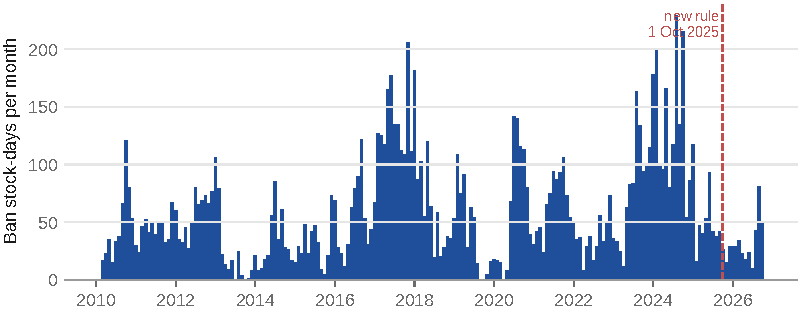
\includegraphics[width=\linewidth]{fig_ban_month}
\exsource{Source: NSE securities-in-ban lists; author's calculations.}
\end{figure}

\section{The basis}
For each stock and day, the basis is computed from the volume-weighted average prices of the future and of the stock, net
of dividends going ex before expiry and of carry at the three-month interbank rate:
\[ m_{it}=\ln\bar F_{it}-\ln\big(\bar S_{it}-\mathrm{PV}_{it}(D)\big)-r_t\tau_{it}. \]
The near-month contract is used, switching to the next month when three or fewer trading days remain; at least five
contracts must trade; contracts with a dividend or other corporate event in their life and the first 20 trading days after
a stock enters the F\&O segment are excluded; the basis is winsorised at 1\% and 99\% within each year. The resulting sample
has 486,040 stock-days for 371 stocks, 8,851 of them in a ban. Its median basis is $+1.1$\bp, and the 10th and 90th
percentiles are $-39.1$ and $+26.8$\bp: the lower tail is wider than the upper (Figure~\ref{fig:basisdist}), as expected
when reverse arbitrage is costlier than cash-and-carry. The basis shrinks toward expiry.

\begin{figure}[t]
\caption[Distribution of the futures-cash basis]{The basis is centred near zero with a long lower tail}\label{fig:basisdist}
\exsub{Basis of the analysis sample, 2015 to 2026, in basis points (3.1\% of stock-days lie beyond 100\bp\ from zero and are not drawn)}
\centering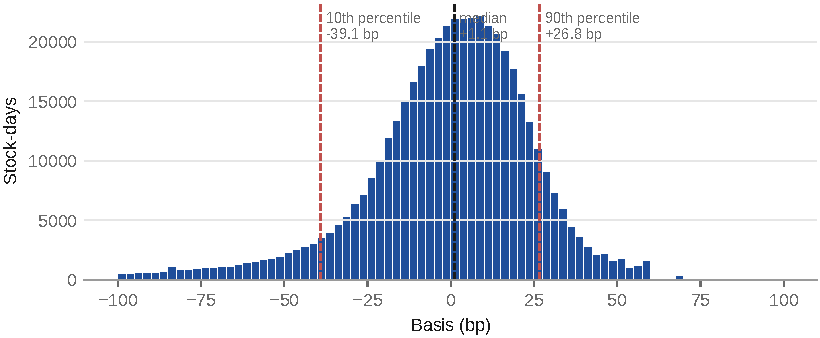
\includegraphics[width=\linewidth]{fig_basis_dist}
\exsource{Source: NSE F\&O and cash bhavcopies, corporate actions, three-month interbank rate; author's calculations.}
\end{figure}
 A relative implied repo rate (the stock's implied financing rate minus the day's cross-sectional median) and a
basis built from closing prices are used as checks.

\section{Other outcomes}
\begin{itemize}
\item \emph{Trading:} futures contracts traded (near and next month), the change in open interest in contracts, the ratio
$R=(\Delta OI+V)/V$, cash volume and the delivery share.
\item \emph{Earnings drift:} the buy-and-hold return over days $+2$ to $+64$ after a results announcement minus that of the
stock's size-decile portfolio; the surprise is the abnormal return over days $-1$ to $+1$; bad (good) news is the bottom
(top) tercile within each quarter. Returns are adjusted for splits, bonuses and dividends (the exchange's previous-close
field is not), and events with a price below Rs 5 are excluded.
\item \emph{Price delay:} the share of a stock's weekly return variation explained by lagged market returns (Hou and
Moskowitz, 2005), by calendar year.
\end{itemize}

\section{A constraint index for all stocks}\label{sec:index}
To measure how hard arbitrage is in each stock without using the outcomes or the treatments, I build a quarterly index for
all NSE stocks (80,042 stock-quarters, 3,310 stocks, 2015 to 2026) from five frictions: no short channel (not in the F\&O
segment), SLB scarcity (share of days without any SLB trade), the Corwin and Schultz (2012) spread, Amihud (2002)
illiquidity and idiosyncratic volatility. Each is standardised within the quarter, and the index is their first
principal component, which explains 53\% of their variance; all five load positively (0.37 to 0.49) and the loadings are
stable from year to year. The index is persistent (quarter-to-quarter rank correlation 0.90).

\begin{table}[t]
\caption[Validation of the constraint index]{More constrained stocks adjust more slowly, also within stocks and after controlling for size}\label{tab:index}
\exsub{Coefficients per standard deviation of the index, frictions measured before the outcomes}
\small\begin{tabular}{@{}>{\raggedright\arraybackslash\bfseries\color{accent}}p{6.2cm}ccc@{}}
\toprule
\thd{Outcome} & \thd{Per s.d.\ (s.e.)} & \thd{Size-controlled} & \thd{Obs.} \\
\midrule
Price delay, next year (year FE) & $+0.058$ (0.003) & $+0.036$ (0.004) & 15,790 \\
Price delay, next year (stock and year FE) & $+0.032$ (0.005) & $+0.028$ (0.006) & 15,790 \\
Absolute drift after announcements & $+0.023$ (0.001) & $+0.015$ (0.001) & 69,673 \\
Drift after bad news & $-0.008$ (0.001) & $-0.001$ (0.002) & 23,219 \\
Drift after good news & $+0.001$ (0.001) & $+0.001$ (0.002) & 23,095 \\
\bottomrule
\end{tabular}

\exsource{FE: fixed effects. Size control: log market capitalisation for price delay (15,227 stock-years with a market capitalisation); market-capitalisation decile fixed effects for drift. Source: author's calculations.}
\end{table}

More constrained stocks respond more slowly to market news, also within a stock over time and after controlling for size,
and drift more after announcements in either direction (Table~\ref{tab:index}). Without a size control, drift after bad
news, but not good news, is stronger for more constrained stocks; with size-decile fixed effects this asymmetry disappears,
so it reflects the smaller size of constrained stocks rather than the short-sale constraint. These are associations. Within F\&O stocks, the short-channel component does not vary and SLB activity
appears to reflect demand to borrow rather than ease of borrowing, so for the futures-cash band of F\&O stocks I use a
separate F\&O index that adds utilisation of the position limit (Chapter~\ref{ch:band}).
